\section{Characterizing Transnational Detours}
\label{datasets}
In this section, we introduce our measurement methods, challenges in conducting the measurements, and our findings on which countries current traffic traverses.

\begin{figure*}[ht]
\centering
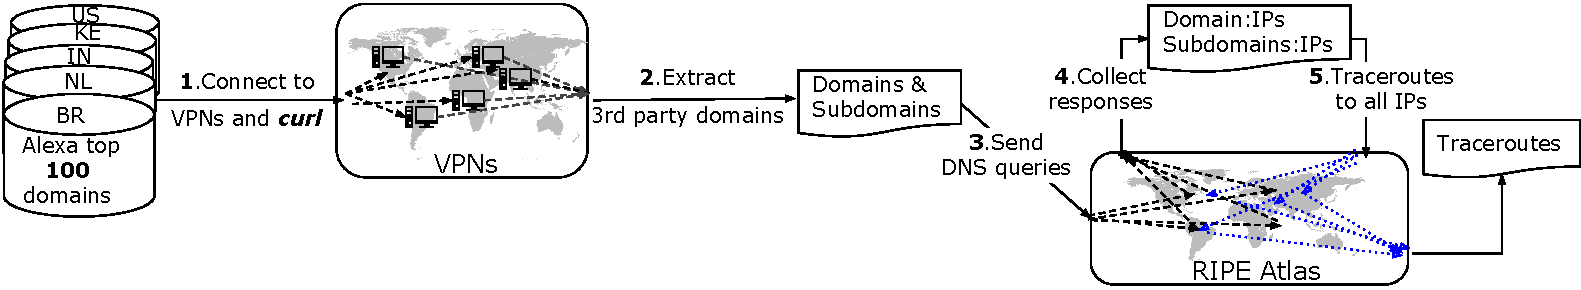
\includegraphics[width=.9\textwidth]{Current-Traffic_fig}
\caption{The measurement pipeline to study current traffic routes.}
\label{fig:pipeline1}
\end{figure*}

\begin{figure}
\centering
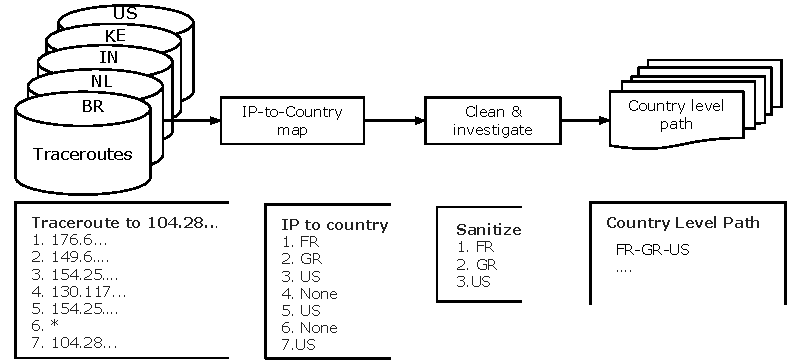
\includegraphics[width=.5\textwidth]{Analysis-Pipeline_fig}
\caption{The measurement pipeline to analyze traceroutes.}
\label{fig:analysis_pipeline}
\end{figure}

\subsection{Measurement Pipeline}
\label{pipeline}
We use the data plane to measure traffic paths; we analyze the reported hops of traceroute measurements to find which countries are on the path from a client in a particular country to a popular domain.  The reverse path is just as important as the forward path, and often the reverse path is different from the forward path; we measure how symmetric the forward and reverse paths are the country-level in Section \ref{path_sym}, and also explain how the exclusion of the reverse path provides a lower bound on the number of countries that traffic traverses.  Using traceroutes to measure transnational detours is new; prior work used BGP routing tables to \textit{infer} country-level paths~\cite{karlin2009nation}.  Because we conduct active measurements, which are limited by our resources, we make a tradeoff and study five countries, as opposed to all countries' Internet paths.  Figure \ref{fig:pipeline1} shows the steps taken for this measurement; first we identify a set of popular domains, then we use RIPE Atlas probes to query DNS with these domains, and traceroute to the DNS responses.  The measurements were conducted on January 31st, 2016.  Our analysis involves the steps seen in Figure \ref{fig:analysis_pipeline}; we map traceroutes to country-level paths.

\subsubsection{Resource Limitations}
\label{resource_limits}
To our knowledge, the publicly available traceroute datasets suitable for our goal are from iPlane~\cite{madhyastha2006iplane} and CAIDA (Center for Applied Internet Data Analysis)~\cite{caida}.  The iPlane project uses PlanetLab~\cite{planetlab} nodes to run traceroutes to all unique AS-level paths in the BGP routing table.  This project also has historical data as far back as 2006.  Unfortunately, because iPlane uses PlanetLab nodes, which have been shown to mostly use the Global Research and Education Network (GREN), the traceroutes from PlanetLab nodes will not be representative of typical Internet users' traffic paths~\cite{banerjee2004interdomain}.  The other publicly available dataset, from CAIDA, ran traceroutes from different vantage points around the world, but to randomized destination IP addresses that cover all /24s.  This is also not sufficient for what we wanted to measure because a typical Internet user is going to access a domain that will be locally resolved; the user will not input a specific IP address in their browser.  

We chose to run active measurements that would be most representative of an Internet user.  We chose to run DNS and traceroute measurements from RIPE Atlas probes, which are hosted all around the world and in many different settings, including home networks~\cite{ripe_atlas}.  RIPE Atlas probes can use the local DNS resolver, which would give us the best estimate of the traceroute destination.

Despite the options RIPE Atlas provides, there were still restrictions that made measurements challenging.  To conduct any measurement on a RIPE Atlas probe, it costs a certain amount of credits, and we were therefore restricted by the number of credits we had.  Additionally, RIPE Atlas imposes rate limits on the number of concurrent measurements and the number of credits that an individual user can spend per day.  We address these challenges in two ways: 1) we reduce the number of necessary measurements we must run on RIPE Atlas probes by conducting traceroute measurements to a single IP address in each /24 (as opposed to all IP address returned by DNS) because all IP addresses in a /24 belong to the same AS, and should therefore be located in the same geographic area; 2) use a different method---VPN connections---to get a vantage point within a foreign country, which is still representative of an Internet user in that country.

\subsubsection{Path Asymmetry}
\label{path_sym}
Previous work has shown that paths are not symmetric most of the time---the forward path from point A to point B does not match the reverse path from point B to point A~\cite{he2005routing}.  Most work on path asymmetry has been done at the AS level, but not at the country level.  Our measurement methods only take the forward path (from client to domain or relay) into account, and not the path from the domain or relay to the client.  

We conducted a study to measure path asymmetry at the country granularity; if country-level paths are symmetric, then the results of our measurements would be representative of the forward {\it and} reverse paths, but if the country-level paths are asymmetric, then our measurement results only provide a lowerbound on the number of countries that could potentially conduct surveillance.  Using 100 RIPE Atlas probes located around the world, and 8 Amazon EC2 instances, we ran traceroute measurements from every probe to every EC2 instance and from every EC2 instance to every probe.  After geolocating the IPs to countries, we analyzed the paths for symmetry.  First, we compared the set of countries on the forward path to the set of countries on the reverse path; this yielded about 30\% symmetry.  What we wanted to know is whether or not the reverse path has more countries on it than the forward path.  We measured how many reverse paths were a subset of the respective forward path; this was the case for 55\% of the paths.  

The results of this measurement are not convincing enough to state that country-level paths are symmetric, and therefore our measurements and results represent a lowerbound on the number of countries that transit traffic; our results are a lowerbound on how many unfavorable countries transit a client's traffic.

\subsubsection{Traceroute Origination and Destination Selection}
As discussed above, we used RIPE Atlas probes in each of the five countries we studied.  Each of these countries had varying amounts of probes hosted in the country, ranging from about 75 probes to many hundreds.  Because of the resource restrictions, we could not use all probes in each of the countries.  We selected the set of probes that had unique ASes in the country to get the widest representation of origination (starting) points.

For destinations, we used the Alexa Top 100 domains in each of the respective countries, as well as the 3rd party domains that are requested as part of an original web request.  To obtain these 3rd party domains we {\tt curl} (fetch) each of the Top 100 domains, but we must do so from within the country we are studying.  There is no current functionality to {\tt curl} from RIPE Atlas probes, so we establish a VPN connection within each of these countries to {\tt curl} each domain and extract the 3rd party domains; we {\tt curl} from the client's location in case web sites are customizing content based on the region of the client.

\subsubsection{Country Mapping}
\label{c_map}
Geolocation services and tools have been studied and proposed, and continue to be a growing research area.  Because that is not the primary focus of our work, we use MaxMind's geolocation service to map IP addresses to their respective countries~\cite{maxmind}.   Our study requires country-level paths, which is a coarser granularity than either city granularity or latitude-longitude granularity.  Previous work has studied the inaccuracy of geolocation services, but the evaluation was at the latitude-longitude granularity~\cite{huffaker2011geocompare}; we observe less inaccuracy at the country-level.  To address the incompleteness of the data, we cleaned up our IP to country mapping by removing all IP addresses that resulted in a `None' response when querying MaxMind, which causes our results to provide a conservative estimate of the number of countries that traffic passes through. It is important to note that removing `None' responses will \textit{always} produce a conservative estimate, and therefore we are \textit{always} underestimating the amount of potential surveillance.  An example of this can be seen in Figure \ref{fig:analysis_pipeline}.  This method provides a lower bound on the number of countries that are included on the path, and therefore a lower bound on the countries that can conduct surveillance.  

\subsection{Results}

%%%% ADD THIS TO datasets.tex
\newcolumntype{d}[1]{D{.}{.}{#1}}
\newcommand{\headrow}[1]{\multicolumn{1}{c}{\adjustbox{angle=45,lap=\width-0.5em}{#1}}}
\newcolumntype{P}[1]{>{\raggedright\arraybackslash}p{#1}}
\newcommand{\ra}[1]{\renewcommand{\arraystretch}{#1}}
\begin{table}[t]
\centering
\ra{1.2}
\resizebox{\columnwidth}{!}{%
\begin{tabular}{@{}ld{3.2}d{3.2}d{3.2}d{3.2}d{3.2}@{}}
%\multicolumn{1}{l}{}    & \headrow{Host} & \headrow{Transit} & \headrow{Host} & \headrow{Transit} &\headrow{Host} &\headrow{Transit} &\headrow{Host}   &\headrow{Transit} &\headrow{Host}  &\headrow{Transit} \\

\textit{Country}    & \headrow{Brazil}  & \headrow{Netherlands}   & \headrow{India} & \headrow{Kenya} & \headrow{United States}\\
\toprule
Brazil             &.169    &-     &-    & -  & - \\ \midrule
Canada             &.001    &.007     &.015      &.006       & -  \\
United States      &\cellcolor[HTML]{F7BE81}.774    &\cellcolor[HTML]{F7BE81}.454      &\cellcolor[HTML]{F7BE81}.629      &\cellcolor[HTML]{F7BE81}.443        &\cellcolor[HTML]{F7BE81}.969    \\ \midrule
France             &.001    &.022      &.009      &.023       &.001 \\
Germany            &.002    &.013      &.014      &.028       &.001  \\
Great Britain      &-  &.019     &.021     &.032       &.002 \\
Ireland            &.016    &.064      &.027       &.108       &.001   \\
Netherlands        &.013    &\cellcolor[HTML]{F7BE81}.392      &.101      &\cellcolor[HTML]{F7BE81}.200      &.024  \\
Spain              &.001    &-     & -    &  -     &-    \\ \midrule
Kenya              &-        &  -    & -    &.022        &-  \\
Mauritius          &  -      & -    & -   &.004       & -  \\
South Africa       & -       & -     & -  &.021       &-  \\ \midrule
United Arab Emirates & -     & -     & -   &.011        &-  \\
India              &  -      & -     &.053    &.002        &-  \\
Singapore          & -       &.002     &\cellcolor[HTML]{F7BE81}.103      &.027       & - \\\hline
\end{tabular}
}
\caption{Fraction of paths that end in each country in default routes.}
\label{tab:host}
\end{table}

\begin{table}[t]
\centering
\ra{1.2}
\resizebox{\columnwidth}{!}{%
\begin{tabular}{@{}ld{3.2}d{3.2}d{3.2}d{3.2}d{3.2}@{}}
%\multicolumn{1}{l}{}    & \headrow{Host} & \headrow{Transit} & \headrow{Host} & \headrow{Transit} &\headrow{Host} &\headrow{Transit} &\headrow{Host}   &\headrow{Transit} &\headrow{Host}  &\headrow{Transit} \\

\textit{Country}    & \headrow{Brazil}  & \headrow{Netherlands}   & \headrow{India} & \headrow{Kenya} & \headrow{United States}\\ \toprule
Brazil              &1.00       & -   & -     & -     & -\\ \midrule
Canada                &.013       &.007     &.016       &.008      &.081 \\
United States        &\cellcolor[HTML]{F7BE81}.844        &\cellcolor[HTML]{F7BE81}.583     &\cellcolor[HTML]{F7BE81}.715      &\cellcolor[HTML]{F7BE81}.616       &\cellcolor[HTML]{F7BE81}1.00 \\ \midrule
France                 &.059     &.102      &.104       &.221      &.104 \\
Germany                 &.005       &.050    &.032      &.048      &.008 \\
Great Britain                &.024       &\cellcolor[HTML]{F7BE81}.140     &\cellcolor[HTML]{F7BE81}.204      &\cellcolor[HTML]{F7BE81}.500      &.006 \\
Ireland                &.028       &.106      &.031     &.133      &.006 \\
Netherlands                 &.019        &1.00      &.121      &\cellcolor[HTML]{F7BE81}.253      &.031 \\\hline
Spain                  &.176       &.004     & -     & -      &- \\ \midrule
Kenya                 & -       &-    & -      &1.00      &- \\\hline
Mauritius                  & -       & -     & -      &\cellcolor[HTML]{F7BE81}.322       &- \\
South Africa                 &-        & -    & -     &\cellcolor[HTML]{F7BE81}.334       &- \\ \midrule
United Arab Emirates                  &.00003        & -    & -     &.152       &- \\
India               &  -    &.0007    &1.00     &.058     &.0005 \\
Singapore                 &.0009        &.002     &\cellcolor[HTML]{F7BE81}.270       &.040       &.003 \\ \midrule
\end{tabular}
}
\caption{Fraction of paths that each country transits in default routes.}
\label{tab:transit}
\end{table}

Table \ref{tab:host} shows the five studied countries along the top of the table, and the countries that host their traffic along the Y axis.  For example, the United States is the endpoint of 84\% of the paths that originate in Brazil.  A ``-'' represents the case where no traffic ended in that country.  For example, no Brazilian paths ended in South Africa. Table \ref{tab:transit} shows the fraction of paths that transit certain countries (along the Y axis).

{\bf Hosting Diversity.}
First we analyzed hosting diversity; this shows us how many unique countries in which a domain is hosted---the more countries that a domain is hosted in creates a greater chance that the content is replicated in a favorable country, and could potentially allow a client to circumvent an unfavorable country.  We queried DNS from 26 vantage points around the world, which are shown in Figure \ref{fig:world}; we chose this set of locations because they are geographically diverse.  We found that about half of the top domains in each of the five countries studied are hosted in more than one country.  Figure~\ref{fig:host_diversity} shows there are two distinct modes in the graph, one representing the domains that are hosted in a single country, and the other mode representing CDNs.  This shows that many domains are hosted in a single unique country, which leads us to our next analysis---where are these domains hosted, and which countries are traversed on the way to reach these locations.

\begin{figure}
\centering
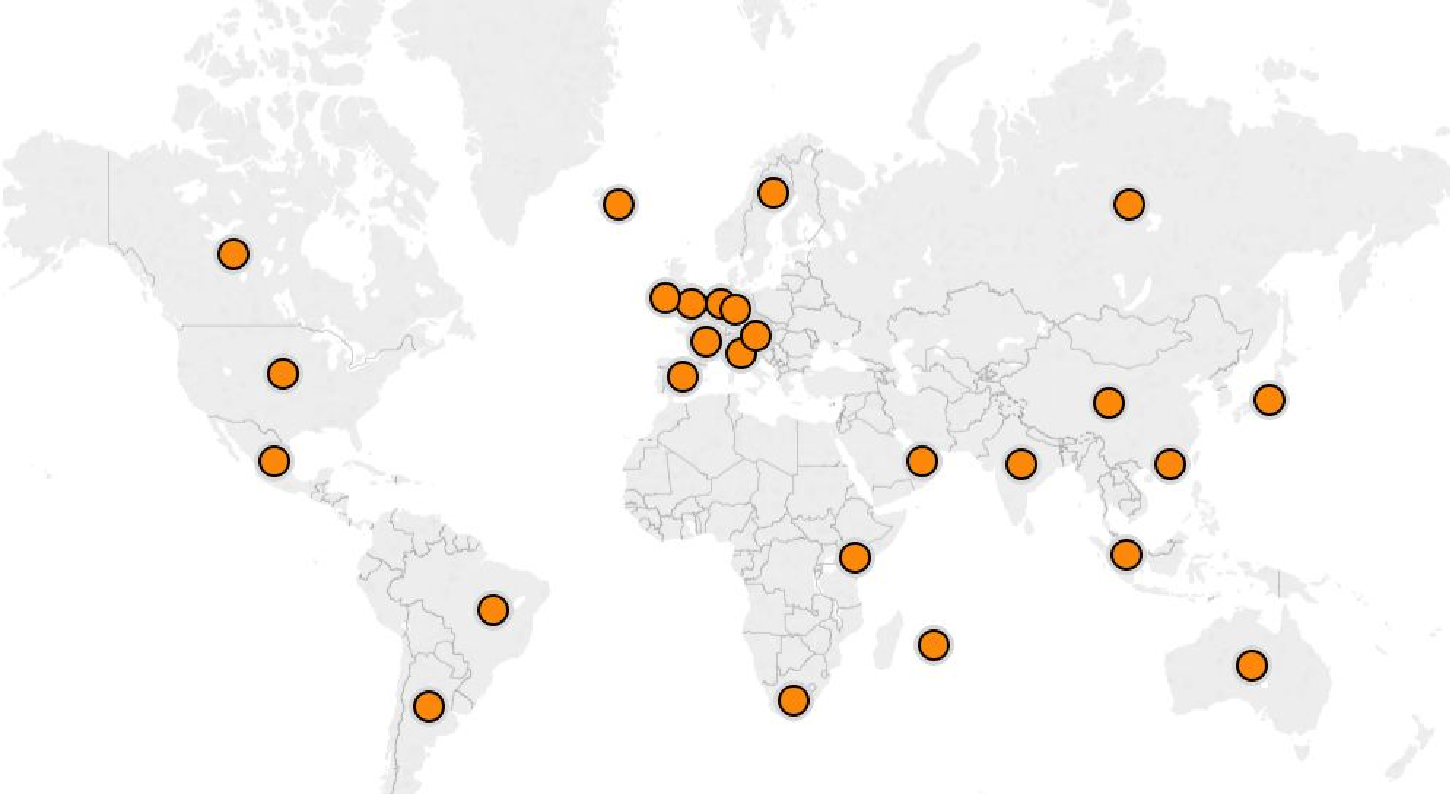
\includegraphics[width=\columnwidth]{World-DNS}
\caption{The locations of vantage points in measuring hosting diversity.}
\label{fig:world}
\end{figure}

\begin{figure}
\centering
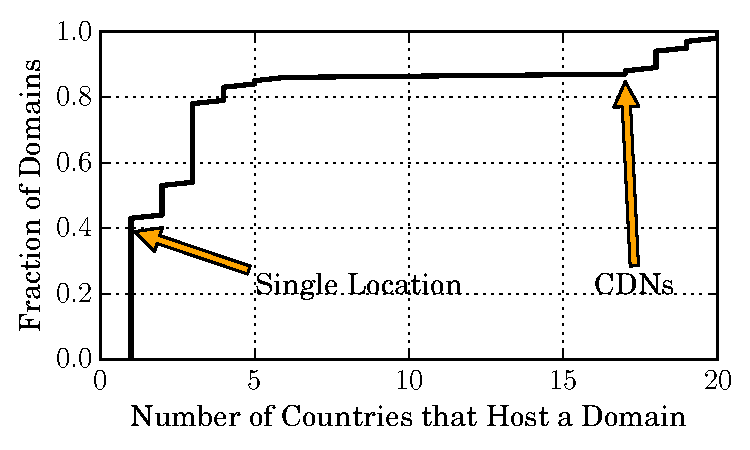
\includegraphics[width=\columnwidth]{domain_hist_US1}
\caption{The number of Alexa Top 100 US Domains hosted in different countries.}
\label{fig:host_diversity}
\end{figure}

{\bf Surveillance States' Host Domains.}
The most common destination among all five countries studied is the United States: 77\%, 45\%, 63\%, 44\%, and 97\% of paths originating in Brazil, Netherlands, India, Kenya and the United States, respectively, are currently reaching content located in the United States. Despite the amount of country-level hosting diversity, we see the majority of paths from all five countries ending in a single country.  The fraction of paths that are hosted in various countries can be seen in Table~\ref{tab:host} (the complete table can be seen in the Appendix).  This is significant because the United States is a known surveillance state, and therefore these percentages represent the amount of foreign traffic that the United States can conduct surveillance on.  Our results also show the Netherlands is a common hosting location for traffic originating in the Netherlands, India, and Kenya.

For Indian traffic, in addition to the 63\% hosted in the United States and the 10\% hosted in the Netherlands, another 10\% is hosted in Singapore.  Hosting in these countries can best be explained by the number of underwater cables with landing points in both India and Singapore~\cite{cablemap}.  More specifically, there is a cable that directly connects Chennai, India and Changi North, Singapore, and is owned by Tata Communications, which is one of the top global Internet providers (in terms of transitted IP space)~\cite{bakers}.  

For Kenyan traffic, the United States hosts 44\% of the content, but Ireland hosts 10\%; Ireland is a popular hosting location for U.S. companies due to its relaxed enforcement of privacy in the private sector \annie{I got this information from Joel Reidenberg - how do I cite that?  I'll also look to see if I can find any publications that discuss this}.  

All of the countries studied (except for the United States) host content for a small percentage of their own traffic.  For traffic that originates in Brazil, only 17\% of it also ends in Brazil.  Only 5\% and 2\% of Indian and Kenyan traffic, respectively, end in the originating country.  

Only a fraction of country code top-level domains are hosted within the respective country.  For Kenya, 24 of the Top 100 Domains are .ke domains, and of these 24 domains only 5 are hosted within Kenya.  29 out of 40 .nl domains are hosted in the Netherlands; 4 of 13 .in domains are hosted in India; 18 of 39 .br domains are hosted in Brazil.  Interestingly, all .gov domains were hosted in their respective country.

{\bf Traffic Transits Surveillance States.}
Similar to the trend of hosting domains, the United States also transits a large portion of foreign traffic---it transits a larger portion of traffic than it hosts.  Brazilian traffic traverses the United States on 84\% of the paths; therefore, the United States can conduct surveillance on 84\% of the traffic originating in Brazil, despite Brazil's strong efforts in avoiding United States surveillance.  Even though India and Kenya are geographically distant, 72\% and 62\% of their traffic transits the United States.  Of the five countries studied, the Netherlands has the lowest percentage of traffic that transits the United States at 58\%.  

Great Britain and the Netherlands are on the path for a significant percentage of traffic originating in India and Kenya.  50\% and 20\% of paths that originate in Kenya and India transit Great Britain.  Traffic that traverses the Netherlands can be explained by the large IXP located there; traffic that traverses Great Britain is likely due to being on the path between the originating country and the final destination in a European country.

Mauritius, South Africa, and the United Arab Emirates transit 32\%, 33\%, and 15\% of traffic from Kenya.  There are direct underwater cables from Kenya to Mauritius, and from Mauritius to South Africa~\cite{cablemap}.  Additionally, there is a cable from Mombasa, Kenya to Fujairah, United Arab Emirates.  This accounts for the large percentages of traffic that pass through these countries.

{\bf Tromboning Traffic Transits Surveillance States.}
As mentioned above, the percentage of domestic traffic in some of the countries studied is extremely small.  For India, only 5\% of traffic is domestic and for Kenya, 2\% is domestic; despite the small amount of domestic traffic, some of this traffic trombones.  This can be seen better in the cases of Brazil and the Netherlands; figure \ref{fig:trombone_netherlands} shows the amount of paths that trombone to different countries for the Netherlands.  Figures \ref{fig:trombone_brazil} and \ref{fig:trombone_kenya} show tromboning Brazilian and Kenyan traffic; despite Brazil's strong efforts in building IXPs to keep local traffic local, we can see that their traffic still trombones to the United States.  This is likely due to the political tension between peers at IXPs \annie{this came from a conversation I had with our nanog shepherd - how do I cite this?  I'll also look into other references on this topic}, which results in fewer peerings with other ASes within Brazil, and more peerings with international ASes. 


\begin{figure*}[t!]
\begin{minipage}{\linewidth}
\begin{subfigure}[b]{.32\linewidth}
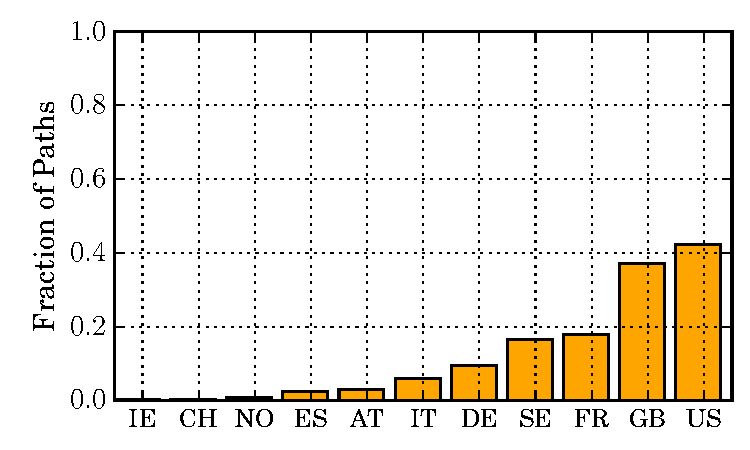
\includegraphics[width=\linewidth]{nl_trombone_new1}
\caption{The countries that tromboning Netherlands traffic transits.\label{fig:trombone_netherlands}}
\end{subfigure}\qquad
\begin{subfigure}[b]{.32\linewidth}
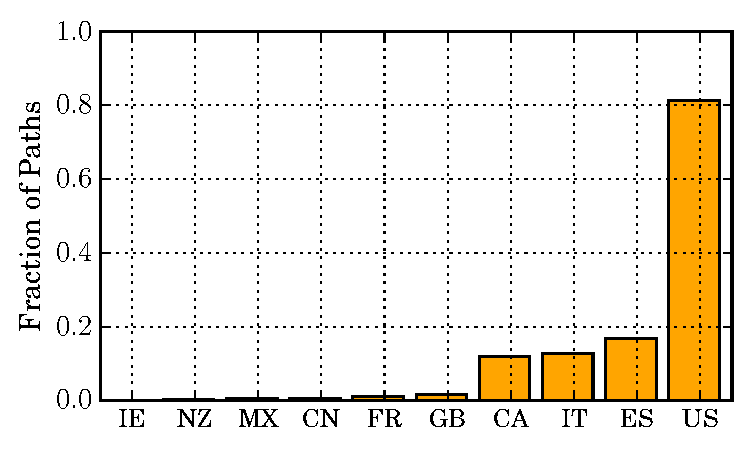
\includegraphics[width=\linewidth]{br_trombone_new1}
\caption{The countries that tromboning Brazilian traffic transits.\label{fig:trombone_brazil}}
\end{subfigure}\qquad
\begin{subfigure}[b]{.32\linewidth}
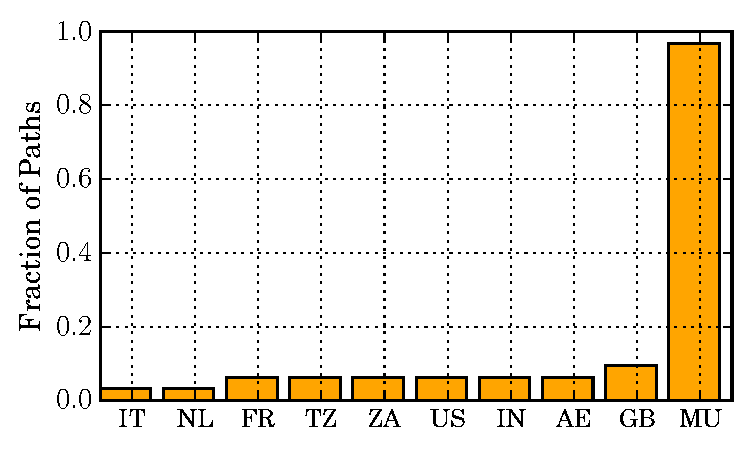
\includegraphics[width=\linewidth]{ke_trombone_new1}
\caption{The countries that tromboning Kenyan traffic transits.\label{fig:trombone_kenya}}
\end{subfigure}
\end{minipage}
\caption{The countries that tromboning traffic from the Netherlands, Brazil, and Kenya transits.}
\label{fig:trombone}
\end{figure*}

%\begin{figure*}[!htb]
%\minipage{0.32\textwidth}
%  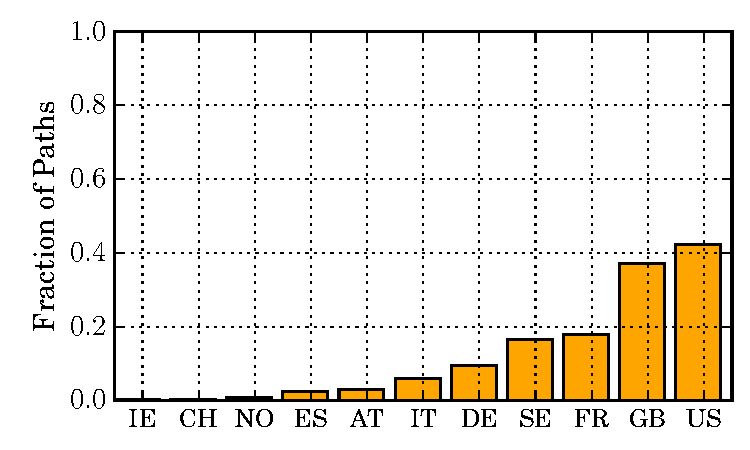
\includegraphics[width=\linewidth]{nl_trombone_new1}
%  \caption{The countries that tromboning Netherlands traffic transits.}\label{fig:trombone_netherlands}
%\endminipage\hfill
%\minipage{0.32\textwidth}
%  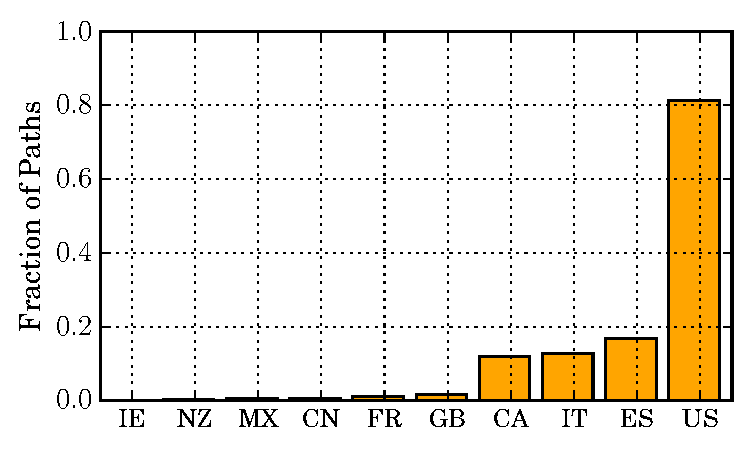
\includegraphics[width=\linewidth]{br_trombone_new1}
%  \caption{The countries that tromboning Brazilian traffic transits.}\label{fig:trombone_brazil}
%\endminipage\hfill
%\minipage{0.32\textwidth}%
%  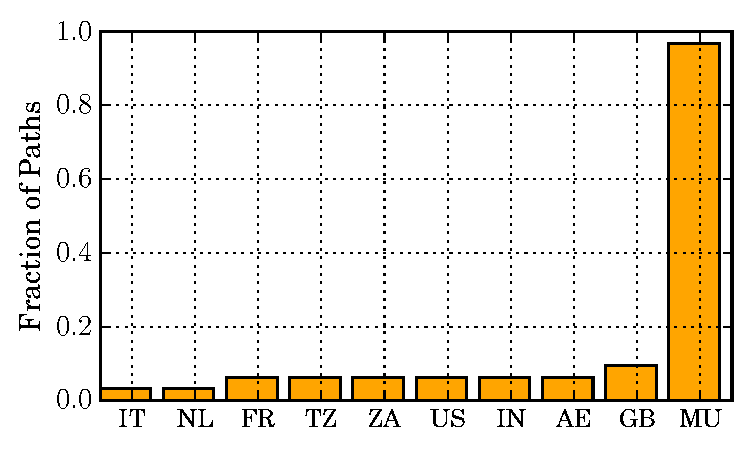
\includegraphics[width=\linewidth]{ke_trombone_new1}
%  \caption{The countries that tromboning Kenyan traffic transits.}\label{fig:trombone_kenya}
%\endminipage
%\end{figure*}

%\begin{figure}
%\centering
%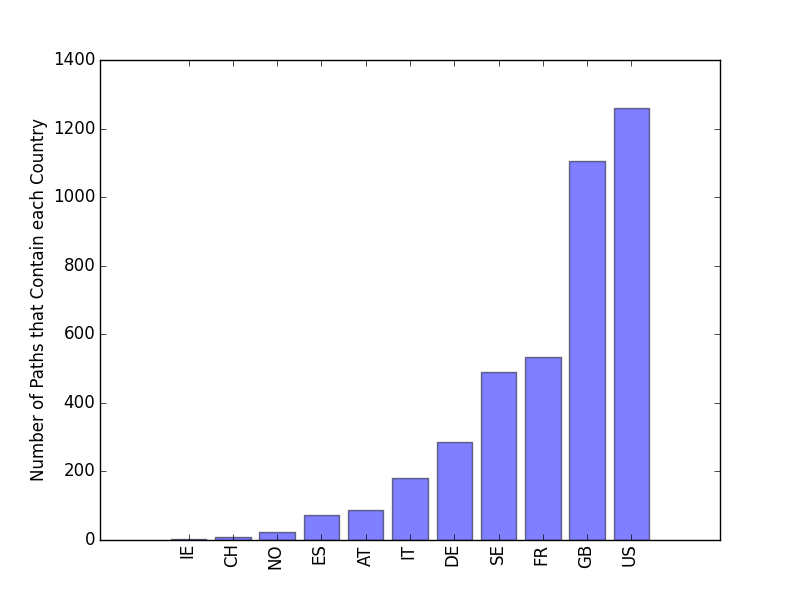
\includegraphics[width=.5\textwidth]{nl_trombone_new}
%\caption{The countries that tromboning Netherlands traffic transits.}
%\label{fig:trombone_netherlands}
%\end{figure}

24\% of all paths originating in the Netherlands (62\% of domestic traffic) trombone to a foreign country before returning to the Netherlands. The most common countries traffic trombones to are the United States and Great Britain.  %Traffic that should be kept local is susceptible to surveillance because it transits two well-known surveillance states.  

{\bf United States as an Outlier.}
Most of the results discussed thus far have shown that Brazilian, Netherlands, Indian, and Kenyan traffic often transit surveillance states, most notably the United States.  The results from studying traffic that originates in the United States are drastically different from those of the other four countries.  The other four countries hosted very small amounts of their own traffic, whereas the United States hosts 97\% of the content that is accessed from within the country.  Only 13 unique countries are ever on a path from the United States to a domain in the top 100 (or third party domain), whereas 30, 30, 25, and 38 unique countries are seen on the paths originating in Brazil, Netherlands, India, and Kenya.  There are only 6 foreign countries---France, Germany, Ireland, Great Britain, and the Netherlands----that host content for traffic originating in the United States, and the fraction of content hosted in these countries is less than 4\% combined.

\subsection{Limitations}
The measurement methods that we described in Section~\ref{datasets} are not without limitations.  First, our study is solely based on IPv4 routes, which likely differ from IPv6 routes.  Here we also discuss limitations with IPv4, country mapping accuracy, and traceroute completeness.

\subsubsection{IPv4}
The measurements we conducted only collect and analyze IPv4 paths, and therefore all IPv6 paths are left out of our study.  IPv6 paths likely differ from IPv4 paths as not all routers that support IPv4 also support IPv6.  Future work includes studying IPv6 paths and which countries they transit, as well as a comparison of country avoidability between IPv4 and IPv6 paths. 

\subsubsection{Country Mapping}
Previous work has shown that there are fundamental challenges in deducing a geographic location from an IP address, despite using different methods such as DNS names of the target, network delay measurements, and host-to-location mapping in conjunction with BGP prefix information~\cite{padmanabhan2001investigation}.  While it has been shown that there are inaccuracies and incompleteness in MaxMind's data~\cite{huffaker2011geocompare}, the focus of this work is on measuring and avoiding surveillance, and not on geolocation algorithms, we therefore used a pre-existing geolocation service. Additionally, we discuss how we address inaccuracies and incompleteness in Section \ref{c_map}.

\subsubsection{Traceroute Accuracy and Completeness}
Our study is limited by the accuracy and completeness of traceroute.  Anomalies can occur in traceroute-based measurements~\cite{augustin2006avoiding}, but most traceroute anomalies do not cause an overestimation in surveillance states.  The incompleteness of traceroutes, where a router does not respond, causes our results to underestimate the number of surveillance states, and therefore also provides a lower bound on surveillance.
